\documentclass{beamer}
\usepackage[utf8]{inputenc}
\usepackage[T1]{fontenc}
\usepackage[swedish,english]{babel}
\usepackage{color}
\usepackage{xcolor}
\usepackage{amssymb}
\usepackage{amsmath}
\usepackage{ae}
\usepackage{units}
\definecolor{olive}{RGB}{0,139,69}
\usetheme{Pittsburgh}
\usecolortheme[RGB={0,139,69}]{structure}
\setbeamertemplate{navigation symbols}{}

\begin{document}

\section{Presentation}

\frame{
  \begin{center}

    \textcolor{olive}{{
        \Large Väderparametrars inverkan på \\ energiförluster i en fastighet
      } \\
      - en studie av värmeflöden
    }

    \vskip10pt

    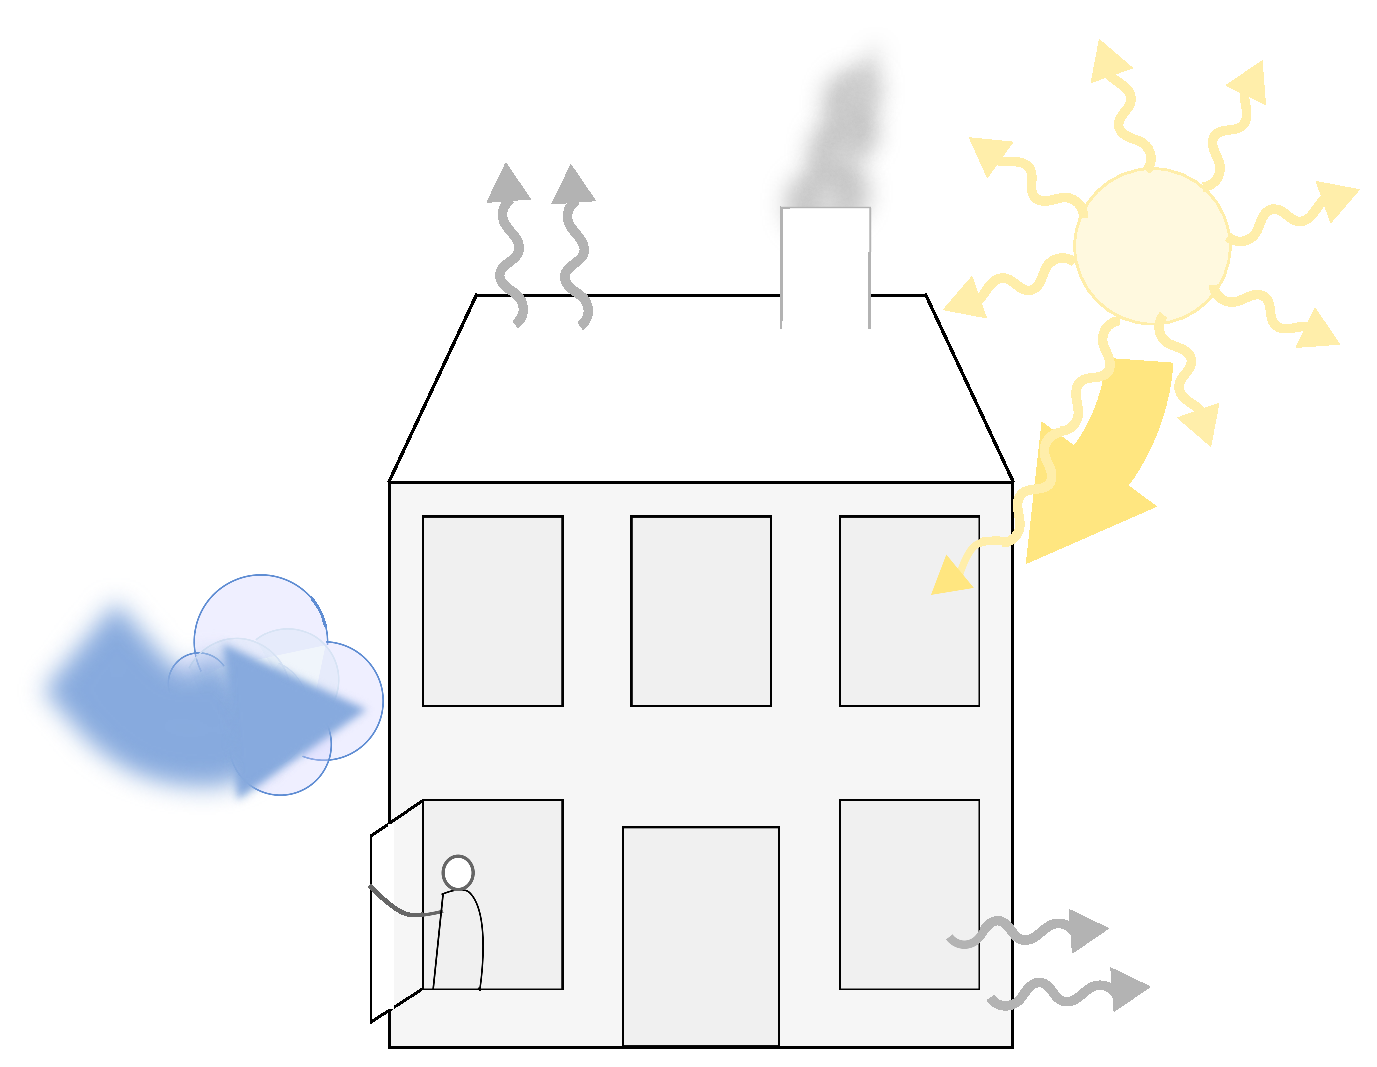
\includegraphics[scale=0.2]{../report/images/hus_framsida.eps}

    \vskip10pt

    Erik Ahlqvist, Ylva Dahl, Mats Lindström, Dan Ståby

    Institutionen för Teknisk Fysik

    29 maj, 2012

  \end{center}

}

\subsection{Byggnadsskal - väggar och tak}

%Definition av h-värde och U-värde

\frame{
       \frametitle{Några definitioner}
        \begin{align*}
        Q &= U\Delta T \\
        Q &= h(T-T_\infty)
        \end{align*}
        \begin{center}
          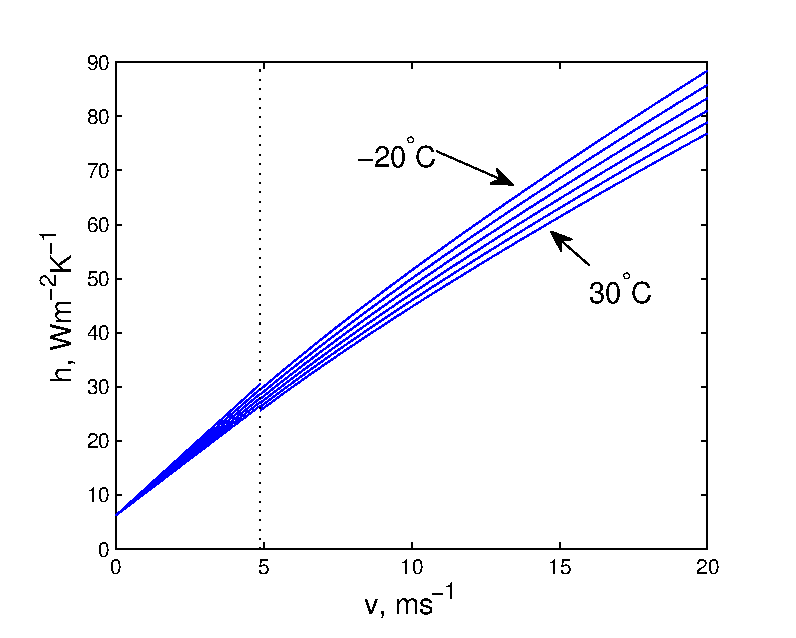
\includegraphics[scale=0.5]{images/hvalues.eps}
        \end{center}
}


%Data för huset

\frame{
       \frametitle{Parametrar för huset}

       \begin{figure}
         \begin{subfigure}[b]{0.48\textwidth}
           \centering
           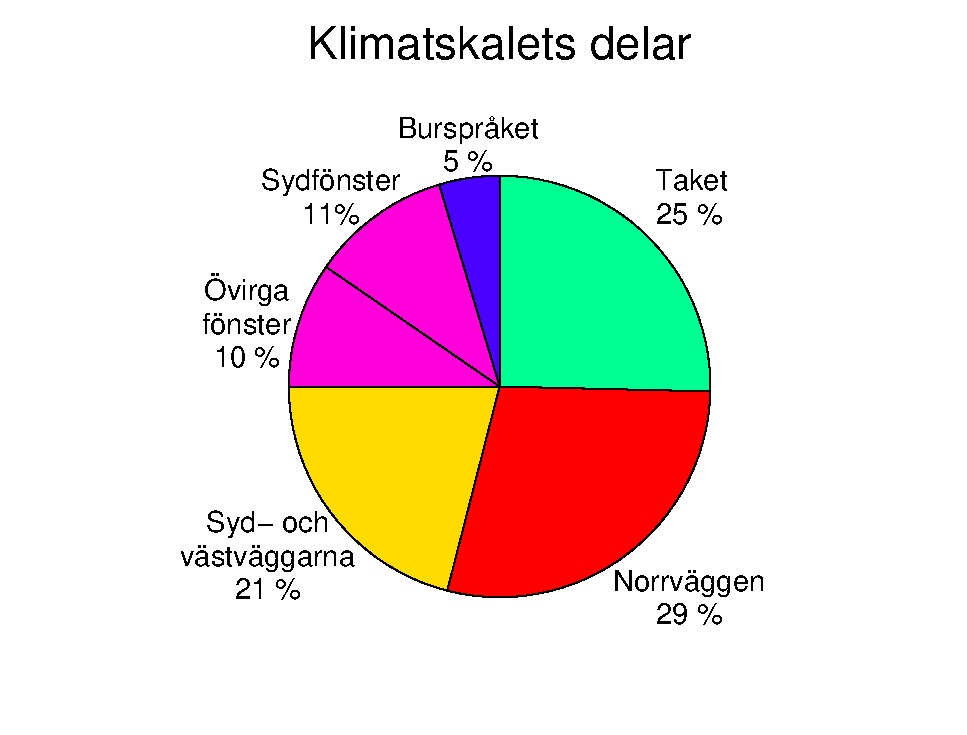
\includegraphics[width=\textwidth]{images/areor_klimatskal.eps}
           \caption*{Total area $\unit[1012]{m^2}$}
         \end{subfigure}
         \begin{subfigure}[b]{0.48\textwidth}
           \centering
           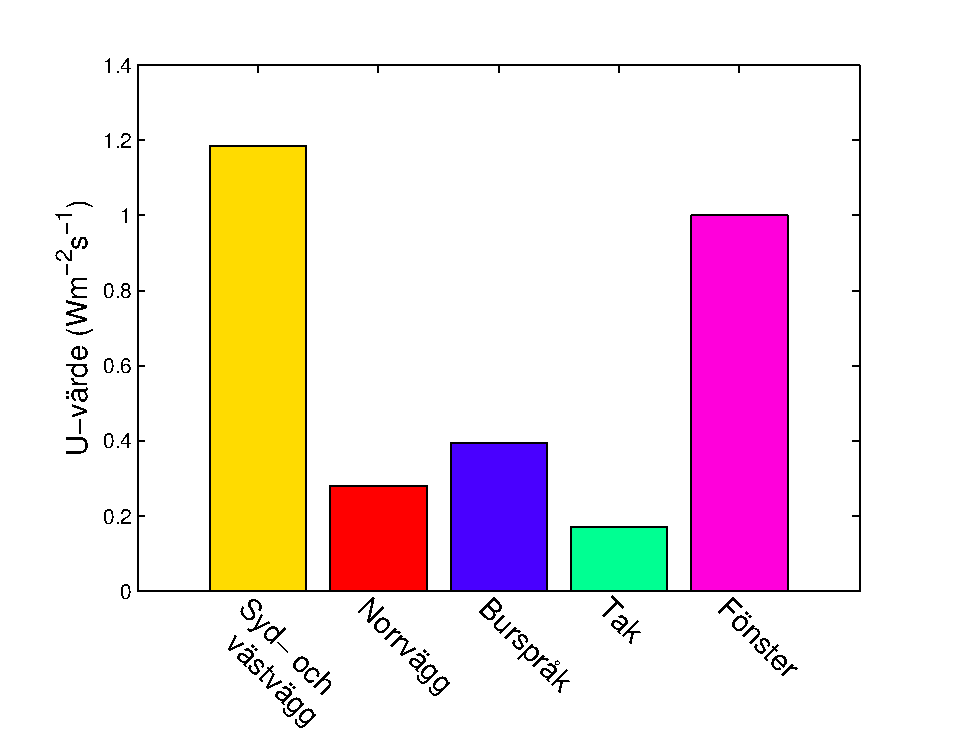
\includegraphics[width=\textwidth]{images/uvalue.eps}
         \end{subfigure}
       \end{figure}
}

\begin{frame}{Problemformulering för väggar och tak}

\begin{align}
k(0)\mathbf{n}\cdot\nabla T(0,t) & = I_{sol}(t) + I_{lv}(T,t) + h(T_\infty-T)
\nonumber \\
T(L,t) & = T_{inne} \nonumber 
\end{align}

\uncover<2>{
\begin{figure}[hbp!]
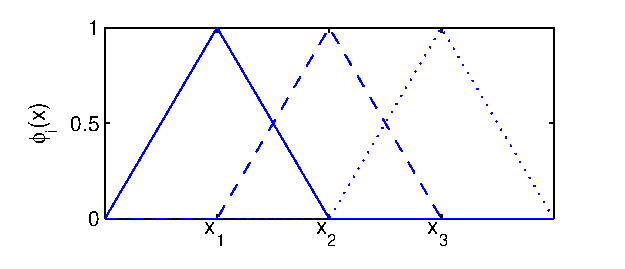
\includegraphics{images/basefun.eps}
\end{figure}
}

\end{frame}

\begin{frame}{Energiflöden, väggar och tak\\En klar decemberdag}
 
\begin{figure}
        \begin{subfigure}[b]{0.48\textwidth}
                \centering
                \includegraphics[width=\textwidth]{images/walls1.eps}
        \end{subfigure}
	\uncover<2>{
        \begin{subfigure}[b]{0.48\textwidth}
                \centering
                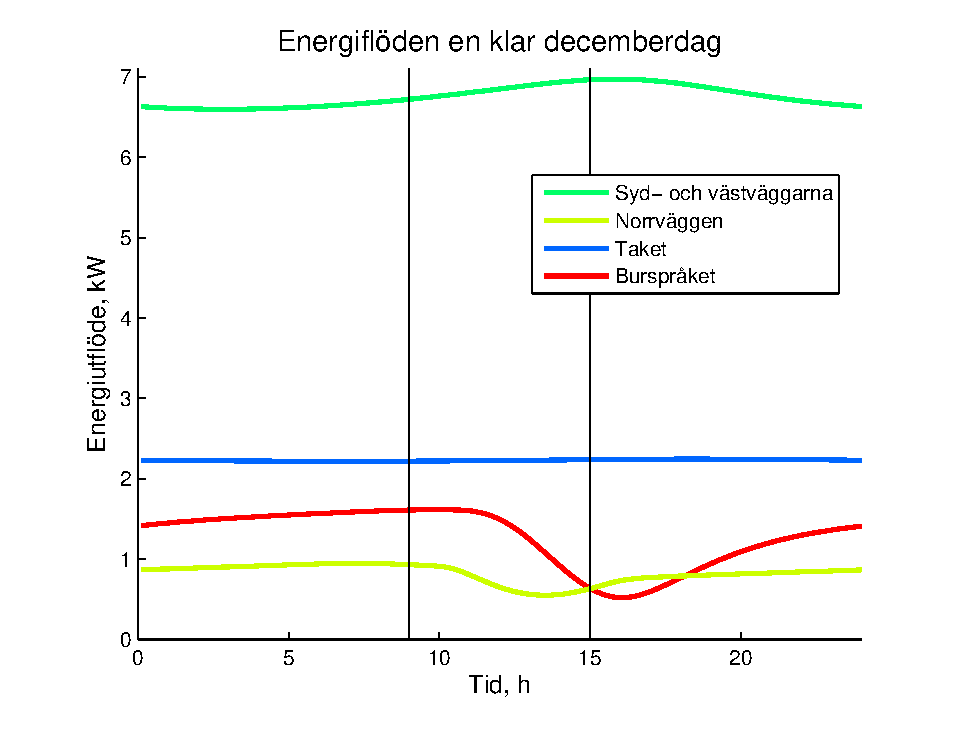
\includegraphics[width=\textwidth]{images/walls2.eps}
        \end{subfigure}
        }
\end{figure}


\end{frame}



\begin{frame}{Infiltrationsförluster}

\begin{figure}[hpbt]
\centering
\includegraphics[width=90mm]{images/pressure3ms.eps}
\caption{\label{fig:windpressure}Vind $\unit[3]{m~s^{-1}}$}
\end{figure}

\end{frame}


\end{document}
